\documentclass[dvips,ruledheader]{abnt}
\usepackage[brazil]{babel}
\usepackage[latin1]{inputenc}
\usepackage[pdftex]{graphicx}
% \usepackage[pdftex]{hyperref}
\usepackage{abnt-alf}
\usepackage{latexsym}
\usepackage{psfrag}
\usepackage[center]{caption2}
% \usepackage{epigraph}

% Gloss�rio n�o utilizado
% \usepackage{makeglo}
% \renewcommand{\glossaryname}{Gloss�rio}
% \makeglossary

\begin{document}

\DeclareGraphicsRule{.eps.gz}{eps}{.eps.bb}{`gunzip -c #1}

% \include{encardenacao}
%	Elemento obrigatório, é a cobertura que reveste o trabalho e 
% deve conter informações de identificação da obra, na seguinte ordem (ANEXO AA):
% · nome da instituição (opcional);
% · nome do autor;
% · título;
% · subtítulo (se houver);
% · número de volumes (se houver mais de um, deve constar, em cada capa, 
%  a especificação do respectivo volume);
% · local (cidade) da instituição onde deve ser apresentado;
% · ano de depósito (da entrega).
\capa
% \mackenzieCapa
\folhaderosto

\tableofcontents

% \include{pre_introducao}
% % ---------------------------------------------------------------------------------------------------- %
%					ORIENTA��ES
% ---------------------------------------------------------------------------------------------------- %
% 	� a apresenta��o sucinta e objetiva do trabalho, fornecendo informa��es sobre sua natu-
% reza, import�ncia e crit�rios de elabora��o, tais como: objetivos, m�todos e procedimen-
% tos seguidos.
% Lendo a introdu��o, o leitor deve sentir-se esclarecido a respeito do conte�do do trabalho,
% assim como do racioc�nio que foi desenvolvido.
% ---------------------------------------------------------------------------------------------------- %

\chapter{Introdu��o}

% ---------------------------------------------------------------------------------------------------- %
%					ORIENTA��ES
% ---------------------------------------------------------------------------------------------------- %
%	Na introdu��o voc� deve retomar os itens do projeto e deixar bem claros: tema, objetivos, 
% justificativa, metodologia e se poss�vel, quais ser�o os cap�tulos, ou seja, comentar o sum�rio, 
% apresnetando o que far� em cada cap�tulo.
% ---------------------------------------------------------------------------------------------------- %

O rootkit � uma ferramenta utilizada em geral por atacantes avan�ados com fins maliciosos e oferece grande obst�culo para ser detectado justamente por ser furtivo e sofisticado recurso de controle de sistemas operacionais.
Seu uso for�a o perito a ter um conhecimento amplo e usar t�cnicas tamb�m sofisticadas para investiga-lo.
Logo entender o seu funcionamento � determinante para uma pericia bem sucedida. 

Esta monografia apresenta uma incurs�o na antiforense focada na utiliza��o de rootkits em ambientes \emph{Microsoft Windows}, visando mostrar o que � um rootkit e os principais empecilhos que o perito pode encontrar ao analis�-lo. 
Para desenvolver esse tema foi utilizada vasta bibliografia e refer�ncias reais para melhor entendimento das t�cnicas de antiforense computacionais utilizadas ou idealizadas que podem ser utilizados por rootkits.

\section{Justificativa}

% ---------------------------------------------------------------------------------------------------- %
%					ORIENTA��ES
% ---------------------------------------------------------------------------------------------------- %
% 	Na justificativa busca-se colocar, de maneira clara e objetiva, quais s�o os elementos 
% te�rico-pr�ticos que demonstram a relev�ncia para a realiza��o da pesquisa, bem como as poss�veis 
% contribui��es resultantes do trabalho proposto.
% ---------------------------------------------------------------------------------------------------- %

Conforme o mundo digitalizou-se, digitalizaram-se tamb�m as suas amea�as, onde antes se podia ver mesmo que por instantes m�sseis ou bombas sendo lan�ada hoje temos in�meras amea�as invis�veis que podem causar tanto estrago quanto, contudo na luz do princ�pio de Locard que diz que tudo que � tocado deixa vest�gios, talvez essas amea�as n�o sejam t�o invis�veis.
O perito deve estar preparado para a a��o de um usu�rio avan�ado que conhe�a bem o sistema operacional atacado, comprometido ou usado.
Mesmo que n�o seja algo corriqueiro na rotina da grande maioria dos profissionais, encontrar um atacante de alto n�vel trar� novos desafios e obst�culos t�o pouco corriqueiros quanto.
Saber como dificultar ou impossibilitar o trabalho do perito � como ele poder� evitar a armadilha de achar que no corpo (corpo de delito) investigado n�o existe nada.

A figura \ref{fig:graph-root} mostra que quantidade de amostras �nicas encontradas de rootkits entre 2009 e 2012 por trimestre nunca foi abaixo de 100 mil.
Esses dados indicam que rootkits s�o amea�as reais e constantes. 
Estudar seu comportamento e entender como ele pode ser usado na antiforense, permite ao perito lidar corretamente com rootkits.

\begin{figure}[htb]
  \centering
  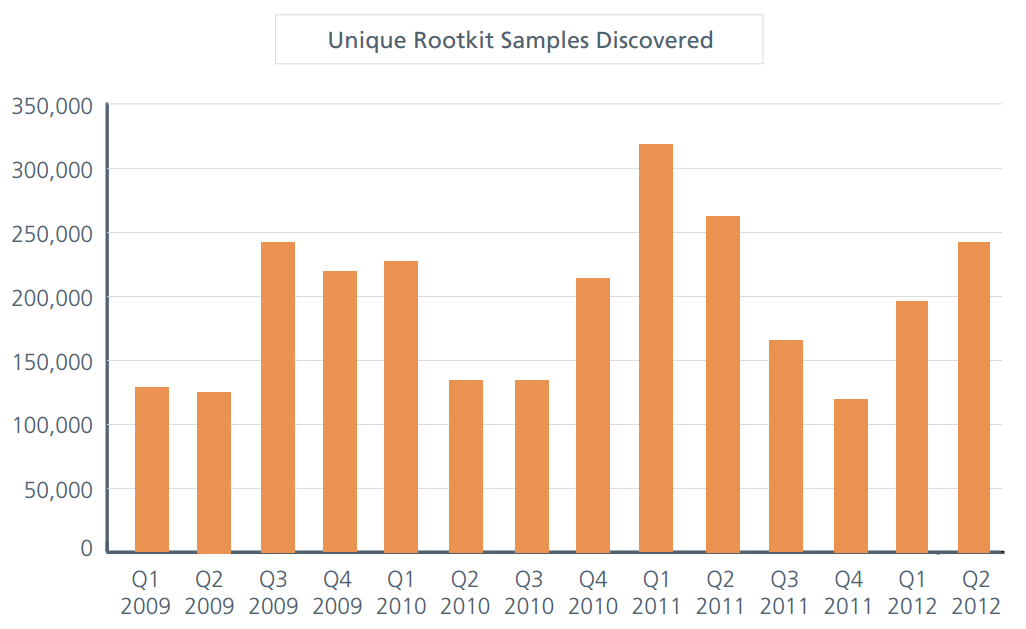
\includegraphics[scale=0.5]{figuras/graph-root.png}
  \caption{Amostras Rootkit �nicas Descobertas \cite{MCAFEE2012}}
  \label{fig:graph-root}
\end{figure}

Com um processo bem definido o perito tende a diminuir o tempo de an�lise e um melhor aproveitamento das mesmas.
Sendo assim, esse trabalho poder� ajudar a tra�ar um processo bem elaborado de trabalho que seja r�pida e eficiente sem deixar brechas que permitam ou ajudem a��es antiforenses provendo mais qualidade com mais precis�o.

\section{Objetivos}

% ---------------------------------------------------------------------------------------------------- %
% Que problemas o estudo do tema pode resolver? (PREPARA��O PAR AO PROBLEMA DE PESQUISA E OBJETIVO)}
% ---------------------------------------------------------------------------------------------------- %

Esse estudo pode ajudar a esclarecer diversos t�picos obscuros a respeito do que pode ser encontrado em investiga��es forenses computacionais quando o perito se v� diante de amea�as persistentes e elaboradas como um rootkit e consequentemente pode ajudar a resolver casos onde foram feitas antiforense.

\subsection{Objetivo Geral}

% ---------------------------------------------------------------------------------------------------- %
%					ORIENTA��ES
% ---------------------------------------------------------------------------------------------------- %
%	� necess�rio apresentar o objetivo geral da pesquisa, ou seja, a meta proposta para a investiga��o, 
% que deve ser coerente com a quest�o de pesquisa.
% ---------------------------------------------------------------------------------------------------- %

Apresentar um processo para an�lise \emph{post mortem} de computadores com Microsoft Windows e as principais t�cnicas antiforense que podem ser encontradas em cada fase do processo.

\subsection{Objetivo Espec�fico}

% ---------------------------------------------------------------------------------------------------- %
%					ORIENTA��ES
% ---------------------------------------------------------------------------------------------------- %
%	De forma complementar, os objetivos espec�ficos, tamb�m presentes nesse item, constituem as etapas 
% de trabalho que permitem alcan�ar o objetivo geral. Como os objetivos traduzem a��es que ser�o executadas 
% ao longo da pesquisa; a apresenta��o destes no texto requer a utiliza��o de verbos no infinitivo.
% ---------------------------------------------------------------------------------------------------- %
Segue os objetivos espec�ficos utilizados para alcan�ar o objetivo principal:

\begin{itemize}
  \item Apresentar o que � ci�ncia forense, para que serve a ci�ncia forense e a legisla��o que garante a exist�ncia do perito no Brasil;
  \item Expor o que � um rootkit, seu funcionamento e seus tipos;
  \item Mostrar o que � antiforense computacional categorizando seus tipos; e
  \item Apresentar um processo de an�lise de rootkit.
\end{itemize}
 
\section{Descri��o dos Cap�tulos}

Ao longo dos cap�tulos s�o desenvolvidos os conhecimentos para o entendimento do tema proposto, onde cada um foi dividido em um assunto espec�fico.

No cap�tulo \emph{Ci�ncia Forense Computacional}, ser� mostrado uma vis�o geral do que � a ci�ncia forense, como ela � aplicada na computa��o, o que � um perito forense computacional e o respaldo legal para sua atua��o.

No cap�tulo \emph{Rootkit}, conduz a uma vis�o do funcionamento de um rootkit, algumas t�cnicas para subverter os sistema, o que � um \emph{malware}, a origem do nome rootkit, o que significa ser o usu�rio \emph{root}, os objetivos do rootkit, suas premissas e sua defini��o.
Tamb�m ser� mostrado os tipos de rootkits e analisado duas categorias gerais que exemplificam como o rootkit pode se manter oculto.

Por fim no �ltimo cap�tulo \emph{An�lise de Rootkits}, ser� apresentado um processo de an�lise \emph{post mortem} com passos que ir�o mostrar em cada etapa o que deve ser feito, t�cnicas antiforense e o qu�o complicado e impactante ela �.

% \section{Metodologia}
% \section{descricao dos capitulos} 

%Peritos em sua nobre luta di�ria podem se deparar, em uma das suas pr�ximas empreitadas t�o ut�is para a sociedade, com algum artefato que tenham sido subvertido por algu�m com o mesmo ou um maior conhecimento do que o seu sobre o corpo de delito periciado.

%Portando em assuntos que fojem da mediocridade cotidiana e adentram nesse mundo instigante e revelador da an�lise de artefatos �nicos, se faz necess�rio que quanto maior o desafio, maior dever� ser a dedica��o e paix�o do perito.

% O perito deve precaver-se de supor que situa��es mais corriqueiras tenham s� e apenas a resposta mais obvia desse modo evitando que sejam subestimadas.
% Al�m do conhecimento t�cnico e de foro que se espera de um perito, compreender que existem t�cnicas sofisticadas para destruir e/ou dificultar acesso a provas no ambito computacional � de fundamental necessidade para qualquer perito. 
% A combina��o do uso de diversas t�cnicas avan�adas com maestria se mostra realmente desafiadora, pois quando isso ocorre o artefato investigado pode estar preparado para ser investigado removendo rastros e evitando a cri��o de evid�ncias.
\chapter*{Objetivo}

$\lombadassss_teste$

\lombada

% \include{cibercrime}
% \include{arquitetura}
% \include{metodologia}
% \include{prevencao}
% \include{legislacao}
% \include{forense} At� aqui revisado
% \include{combate}
% \include{produtos}
% \include{roadmap}
% \include{cases}
% \include{vantagens_desvantagens}
% \include{concorrentes}
% \include{recuperacao_perdas}
% \chapter{Conclusão}
nao existe tecnica antiforense 100\% nem metodologia para analise infalivel, nem 100\% segura e confiavel. foi mostrado diversas técnicas para atrasar e confundir o perito, e por vezes tornando o tempo de análise tao grande que o mesmo nao poderia 

% referencias

\href{http://www.fraudes.org/recupera.asp}{Perdas e Recupera��o}
\href{http://mariano.delegadodepolicia.com/tag/pcc}{Pesquisar crime organizado brasileiro ligado ao cibercrime}

% legisla��o
% ISO: http://www.27000.org
% Paper do Coriolano: http://www2.oabsp.org.br/asp/comissoes/sociedade_informacao/artigos/crimes_ciberneticos.pdf
% Projeto de Lei 2126/2011: http://www.camara.gov.br/proposicoesWeb/fichadetramitacao?idProposicao=517255
% PCC e CV: http://mariano.delegadodepolicia.com/tag/pcc
% Marco civil: http://culturadigital.br/marcocivil/2011/10/27/marco-civil-encaminhado-ao-congress/


\href{http://icommercepage.wordpress.com/2009/07/12/classificacao-dos-crimes-digitais/}
\href{http://convergenciadigital.uol.com.br/cgi/cgilua.exe/sys/start.htm?infoid=16378\&sid=17}
\href{http://pingado.terra.com.br/noticias/57825/tecn-da-informacao/antonio-gesteira-presidente-da-nfe-do-brasil-preve-aumento-da-fiscalizacao-da-receita-fe.html}
\href{http://www1.folha.uol.com.br/folha/informatica/ult124u19455.shtml}{Juliana Carpanez - Folha Online}
\href{http://cartilha.cert.br/fraudes/}
\href{http://www.fraudes.org/}
\href{http://www.valorizeseudinheiro.com.br/dicas-para-evitar-fraudes-em-cheques/}
\href{http://forensedigital.com.br/new/o-mercado-negro-do-cibercrime-em-expansao/}
\href{http://www.fbi.gov/about-us/investigate/cyber/cyber}
\href{http://www.ic3.gov/default.aspx}
\href{http://www.tecmundo.com.br/conexao/3486-conheca-os-cybercrimes-e-aprenda-a-se-defender-deles.htm}
\href{http://mariano.delegadodepolicia.com/category/artigos/}
\href{http://www.nytimes.com/2003/10/27/business/technology-brazil-becomes-a-cybercrime-lab.html?pagewanted=all&src=pm}
\href{http://nakedsecurity.sophos.com/2011/10/05/brazils-cybercrime-evolution-it-doesnt-look-pretty/}
\href{http://idgnow.uol.com.br/internet/2007/05/11/idgnoticia.2007-05-10.5490328067/paginador/pagina_5}
\href{http://www.fraudeseletronicas.com.br/}
\href{http://jus.com.br/revista/texto/2250/crimes-de-informatica}
% \href{http://imasters.com.br/artigo/9741/forense/google_forensics_investigando_cybercrimes}
\href{http://forensedigital.com.br/new/o-mercado-negro-do-cibercrime-em-expansao/}
\href{http://itweb.com.br/53372/orgaos-legais-detectam-5-vezes-mais-casos-de-cibercrime-em-2011/}
\href{http://www.slideshare.net/fullscreen/Trustwave/executive-summary-trustwave-2012-global-security-report/1}


MODUS OPERANDI

\href{http://www.drtomoconnor.com/3100/3100lect04.htm}{}


ESTAT�STICA

\href{http://www.crimecibernetico.com.br/} {}
% \href{http://www.relatoriobancario.com.br/rb/noticias/cielo_fecha_parceria_para_prevencao_de_fraudes_eletronicas}{}

COMBATE

\href{http://olhardigital.uol.com.br/negocios/digital_news/noticias/lei_de_crimes_na_internet_entenda_as_principais_polemicas_em_torno_do_projeto}
\href{http://www.cmsoftware.com.br/produto-neural-risk-persona-fraud-free.asp}
\href{http://olhardigital.uol.com.br/negocios/digital_news/noticias/fraudes_eletronicas_bancarias_geraram_perdas_de_r_685_milhoes_no_semestre}
\href{http://www.rac.com.br/institucionais/cenario-xxi/2005/02/26/3193/cpqd-e-cerebrus-se-aliam-contra-fraudadores}{}

FRAUDES

\href{http://www.decisionreport.com.br/publique/cgi/cgilua.exe/sys/start.htm?infoid=8136&sid=42}{}

PERDAS FINANCEIRAS

\href{http://www.febraban.org.br/Noticias1.asp?id_texto=1321}{}

CEN�RIO ATUAL

\href{http://www2.oabsp.org.br/asp/comissoes/sociedade_informacao/artigos/crimes_ciberneticos.pdf}{}


FILMES RECOMENDADOS

\begin{itemize}
  \item[$\bullet$]Catch Me If You Can (2002) ? [Prenda-me se for capaz]
  \item[$\bullet$]Fun with Dick and Jane ? [Jick \& Jane]
  \item[$\bullet$]Trakedown - [Filme sobre o Mitnik]
\end{itemize}

% \include{glossario}

\bibliography{bb}
\bibliographystyle{abnt-alf}

\end{document}
